\documentclass[lettersize,journal]{IEEEtran}
\usepackage{amsmath,amsfonts}
\usepackage{algorithmic}
\usepackage{array}
\usepackage[caption=false,font=normalsize,labelfont=sf,textfont=sf]{subfig}
\usepackage{textcomp}
\usepackage{stfloats}
% \usepackage{url}
\usepackage{xstring}        % for IEEEtranDOI.bst
\usepackage{verbatim}
\usepackage{graphicx}
\usepackage[noadjust]{cite}
\usepackage[colorlinks=true,urlcolor=blue,linkcolor=blue,citecolor=blue,breaklinks=true,bookmarks=false, pdfpagemode=FullScreen]{hyperref}
\usepackage[table]{xcolor}
% \colorlet{ured}{red!60!gray}
% \colorlet{ured}{red!60!blue}
\colorlet{ured}{black}              % modified version after uni-edit
% \colorlet{rured}{red!60!gray}       % red text for revision
\colorlet{rured}{black}       % red text for revision

\newcolumntype{P}[1]{>{\centering\arraybackslash}p{#1}}
\newcolumntype{M}[1]{>{\centering\arraybackslash}m{#1}}
\def\SPSB#1#2{\rlap{\textsuperscript{#1}}\SB{#2} }
\def\SP#1{\textsuperscript{#1}}
\def\SB#1{\textsubscript{#1}}
\def\mum{\textmu m }
\def\ur#1{{\color{ured}#1}}
\def\rur#1{{\color{rured}#1}}

\hyphenation{op-tical net-works semi-conduc-tor IEEE-Xplore}
\def\BibTeX{{\rm B\kern-.05em{\sc i\kern-.025em b}\kern-.08em
    T\kern-.1667em\lower.7ex\hbox{E}\kern-.125emX}}
\usepackage{balance}
\begin{document}
\bstctlcite{IEEEexample:BSTcontrol}

%............................................................................ main ............................................................................%

%..................................................... title ...........................................................%
\title{\ur{IEEE Photonics Journal Example Using LaTeX}}

%..................... authors and footnotes ...................%
\author{
% 1st
Kuo-Fang Chung, 
\thanks{Manuscript received xx xxx xxxx; revised xx xxx xxxx; accepted xx xxx xxxx. Date of publication xx xxx xxxx; 
date of current version xx xxx xxxx. This work was supported by the Ministry of Science and Technology, 
Taiwan (MOST 110-2224-E-992-001, MOST 111-2119-M-002-009). \\\textit{(Corresponding author: Ding-Wei Huang.)}} \and 
% 2nd
Tien-Tsorng Shih, 
\thanks{Kuo-Fang Chung\ur{, Jiun-Haw Lee}, and Ding-Wei Huang are with \ur{the} 
Graduate Institute of Photonics and Optoelectronics, National Taiwan University, Taipei 106319, Taiwan 
(e-mail: d08941008@ntu.edu.tw; jiunhawlee@ntu.edu.tw; dwhuang@ntu.edu.tw)} \and 
% 3th
Jiun-Haw Lee, 
\thanks{Tien-Tsorng Shih is with \ur{the} 
Department of Electronic Engineering, National Kaohsiung University of Science and Technology, Kaohsiung 807618, Taiwan 
(e-mail: tt@nkust.edu.tw)} \and 
% 4th
and Ding-Wei Huang
\thanks{\ur{Jiun-Haw Lee and Ding-Wei Huang are} also with \ur{the} 
Department of Electrical Engineering, National Taiwan University, Taipei 106319, Taiwan} \and 
\thanks{Digital Object Identifier xx.xxxx/xxx.xxxx.xxxxxxx}
}


%...................... corner stetement (journal information)........................%
\markboth{Journal of \LaTeX\ Class Files,~Vol.~xx, No.~x, xxx~xxxx}%
{How to Use the IEEEtran \LaTeX \ Templates}

\maketitle


%.................................................. abstract ..........................................................%
\begin{abstract}
    %............................................................................ commented ...............................................................................................%
    \begin{comment}
	Test comment
    \end{comment}
    %............................................................................ commented ...............................................................................................%
    Blah, Blah, Blah, Blah, Blah, Blah, Blah, Blah, Blah, Blah, Blah, Blah, Blah, Blah, Blah, Blah, Blah, Blah, Blah, Blah, Blah, 
    Blah, Blah, Blah, Blah, Blah, Blah, Blah, Blah, Blah, Blah, Blah, Blah, Blah, Blah, Blah, Blah, Blah, Blah, Blah, Blah, Blah, 
    Blah, Blah, Blah, Blah, Blah, Blah, Blah, Blah, Blah, Blah, Blah, Blah, Blah, Blah, Blah, Blah, Blah, Blah, Blah, Blah, Blah, 
    Blah, Blah, Blah, Blah, Blah, Blah, Blah, Blah, Blah, Blah, Blah, Blah, Blah, Blah, Blah, Blah, Blah, Blah, Blah, Blah, Blah, 
    Blah, Blah, Blah, Blah, Blah, Blah, Blah, Blah, Blah, Blah, Blah, Blah, Blah, Blah, Blah, Blah, Blah, Blah, Blah, Blah, Blah, 
    Blah, Blah, Blah, Blah, Blah, Blah, Blah, Blah, Blah, Blah, Blah, Blah, Blah, Blah, Blah, Blah, Blah, Blah, Blah, Blah, Blah, 
    Blah, Blah, Blah, Blah, Blah, Blah, Blah, Blah, Blah, Blah, Blah, Blah, Blah, Blah, Blah, Blah, Blah, Blah, Blah, Blah, Blah.
\end{abstract}

\begin{IEEEkeywords}
    Ryan Chung.
\end{IEEEkeywords}


%................................................................ introduction ......................................................%
\section{Introduction}
	\IEEEPARstart{T}{o} meet the demand for higher processing speed and data capacity 
    Blah, Blah, Blah, Blah, Blah, Blah, Blah, Blah, Blah, Blah, Blah, Blah, Blah, Blah, Blah, Blah, Blah, Blah, 
    Blah, Blah, Blah, Blah, Blah, Blah, Blah, Blah, Blah, Blah, Blah, Blah, Blah, Blah, Blah, Blah, Blah, Blah, 
    Blah, Blah, Blah, Blah, Blah, Blah, Blah, Blah, Blah, Blah, Blah, Blah, Blah, Blah, Blah, Blah, Blah, Blah, 
    Blah, Blah, Blah, Blah, Blah, Blah, Blah, Blah, Blah, Blah, Blah, Blah, Blah, Blah, Blah, Blah, Blah, Blah, 
    Blah, Blah, Blah, Blah, Blah, Blah, Blah, Blah, Blah, Blah, Blah, Blah, Blah, Blah, Blah, Blah, Blah, Blah, 
    Blah, Blah, Blah, Blah, Blah, Blah, Blah, Blah, Blah, Blah, Blah, Blah, Blah, Blah, Blah, Blah, Blah, Blah, 
    Blah, Blah, Blah, Blah, Blah, Blah, Blah, Blah, Blah, Blah, Blah, Blah, Blah, Blah, Blah, Blah, Blah, Blah, 
    
    Blah, Blah, Blah, Blah, Blah, Blah, Blah, Blah, Blah, Blah, Blah, Blah, Blah, Blah, Blah, Blah, Blah, Blah, 
    Blah, Blah, Blah, Blah, Blah, Blah, Blah, Blah, Blah, Blah, Blah, Blah, Blah, Blah, Blah, Blah, Blah, Blah, 
    Blah, Blah, Blah, Blah, Blah, Blah, Blah, Blah, Blah, Blah, Blah, Blah, Blah, Blah, Blah, Blah, Blah, Blah, 
    Blah, Blah, Blah, Blah, Blah, Blah, Blah, Blah, Blah, Blah, Blah, Blah, Blah, Blah, Blah, Blah, Blah, Blah, 
    Blah, Blah, Blah, Blah, Blah, Blah, Blah, Blah, Blah, Blah, Blah, Blah, Blah, Blah, Blah, Blah, Blah, Blah, 
    Blah, Blah, Blah, Blah, Blah, Blah, Blah, Blah, Blah, Blah, Blah, Blah, Blah, Blah, Blah, Blah, Blah, Blah, 
    Blah, Blah, Blah, Blah, Blah, Blah, Blah, Blah, Blah, Blah, Blah, Blah, Blah, Blah, Blah, Blah, Blah, Blah, 
    
    Blah, Blah, Blah, Blah, Blah, Blah, Blah, Blah, Blah, Blah, Blah, Blah, Blah, Blah, Blah, Blah, Blah, Blah, 
    Blah, Blah, Blah, Blah, Blah, Blah, Blah, Blah, Blah, Blah, Blah, Blah, Blah, Blah, Blah, Blah, Blah, Blah, 
    Blah, Blah, Blah, Blah, Blah, Blah, Blah, Blah, Blah, Blah, Blah, Blah, Blah, Blah, Blah, Blah, Blah, Blah, 
    Blah, Blah, Blah, Blah, Blah, Blah, Blah, Blah, Blah, Blah, Blah, Blah, Blah, Blah, Blah, Blah, Blah, Blah, 
    Blah, Blah, Blah, Blah, Blah, Blah, Blah, Blah, Blah, Blah, Blah, Blah, Blah, Blah, Blah, Blah, Blah, Blah, 
    Blah, Blah, Blah, Blah, Blah, Blah, Blah, Blah, Blah, Blah, Blah, Blah, Blah, Blah, Blah, Blah, Blah, Blah, 
    Blah, Blah, Blah, Blah, Blah, Blah, Blah, Blah, Blah, Blah, Blah, Blah, Blah, Blah, Blah, Blah, Blah, Blah, 
    \begin{figure}[!t]
		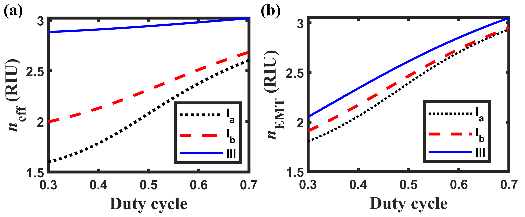
\includegraphics{Fig_sample.pdf}
		\centering
		\caption{\label{fig:MMWBGsche}Schematic \textbf{(a)} 3-D and \textbf{(b)} top views of the proposed MMWBG.}
	\end{figure}
    Blah, Blah, Blah, Blah, Blah, Blah, Blah, Blah, Blah, Blah, Blah, Blah, Blah, Blah, Blah, Blah, Blah, Blah, 
    Blah, Blah, Blah, Blah, Blah, Blah, Blah, Blah, Blah, Blah, Blah, Blah, Blah, Blah, Blah, Blah, Blah, Blah, 
    Blah, Blah, Blah, Blah, Blah, Blah, Blah, Blah, Blah, Blah, Blah, Blah, Blah, Blah, Blah, Blah, Blah, Blah, 
    Blah, Blah, Blah, Blah, Blah, Blah, Blah, Blah, Blah, Blah, Blah, Blah, Blah, Blah, Blah, Blah, Blah, Blah, 
    Blah, Blah, Blah, Blah, Blah, Blah, Blah, Blah, Blah, Blah, Blah, Blah, Blah, Blah, Blah, Blah, Blah, Blah, 
    Blah, Blah, Blah, Blah, Blah, Blah, Blah, Blah, Blah, Blah, Blah, Blah, Blah, Blah, Blah, Blah, Blah, Blah, 
    Blah, Blah, Blah, Blah, Blah, Blah, Blah, Blah, Blah, Blah, Blah, Blah, Blah, Blah, Blah, Blah, Blah, Blah, 
    
    In this \ur{study}, 
    Blah, Blah, Blah, Blah, Blah, Blah, Blah, Blah, Blah, Blah, Blah, Blah, Blah, Blah, Blah, Blah, Blah, Blah, 
    Blah, Blah, Blah, Blah, Blah, Blah, Blah, Blah, Blah, Blah, Blah, Blah, Blah, Blah, Blah, Blah, Blah, Blah, 
    Blah, Blah, Blah, Blah, Blah, Blah, Blah, Blah, Blah, Blah, Blah, Blah, Blah, Blah, Blah, Blah, Blah, Blah, 
    Blah, Blah, Blah, Blah, Blah, Blah, Blah, Blah, Blah, Blah, Blah, Blah, Blah, Blah, Blah, Blah, Blah, Blah, 
    Blah, Blah, Blah, Blah, Blah, Blah, Blah, Blah, Blah, Blah, Blah, Blah, Blah, Blah, Blah, Blah, Blah, Blah, 
    Blah, Blah, Blah, Blah, Blah, Blah, Blah, Blah, Blah, Blah, Blah, Blah, Blah, Blah, Blah, Blah, Blah, Blah, 
    Blah, Blah, Blah, Blah, Blah, Blah, Blah, Blah, Blah, Blah, Blah, Blah, Blah, Blah, Blah, Blah, Blah, Blah, 


\section{Device principle and optimization}
\label{sec:two}
    \begin{figure}[!t]
		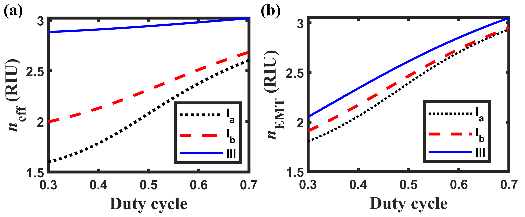
\includegraphics{Fig_sample.pdf}
		\centering
		\caption{\label{fig:vb}Effective refractive indices of the first three TE modes versus core widths for four channel wavelengths.}
	\end{figure}
	Blah, Blah, Blah, Blah, Blah, Blah, Blah, Blah, Blah, Blah, Blah, Blah, Blah, Blah, Blah, Blah, Blah, Blah, 
    Blah, Blah, Blah, Blah, Blah, Blah, Blah, Blah, Blah, Blah, Blah, Blah, Blah, Blah, Blah, Blah, Blah, Blah, 
    Blah, Blah, Blah, Blah, Blah, Blah, Blah, Blah, Blah, Blah, Blah, Blah, Blah, Blah, Blah, Blah, Blah, Blah, 
    Blah, Blah, Blah, Blah, Blah, Blah, Blah, Blah, Blah, Blah, Blah, Blah, Blah, Blah, Blah, Blah, Blah, Blah, 
    Blah, Blah, Blah, Blah, Blah, Blah, Blah, Blah, Blah, Blah, Blah, Blah, Blah, Blah, Blah, Blah, Blah, Blah, 
    Blah, Blah, Blah, Blah, Blah, Blah, Blah, Blah, Blah, Blah, Blah, Blah, Blah, Blah, Blah, Blah, Blah, Blah, 
    Blah, Blah, Blah, Blah, Blah, Blah, Blah, Blah, Blah, Blah, Blah, Blah, Blah, Blah, Blah, Blah, Blah, Blah, 
    \begin{align}
        \frac{\partial B_\text{\textit{\textmu}}}{\partial z} &= j\kappa_\text{dc,\textit{\textmu \textmu}}B_\text{\textit{\textmu}} + 
                j\kappa_\text{ac,\textit{v\textmu}}A_\text{\textit{v}}\cdot \textit{e}^{-j(\Delta \beta z - \phi (z))}\text{,}\label{eq:oneB} \\
        \frac{\partial A_\text{\textit{v}}}{\partial z} &= -j\kappa_\text{dc,\textit{vv}}A_\text{\textit{v}} - 
                j\kappa_\text{ac,\textit{\textmu v}}B_\text{\textit{\textmu}}
                \cdot \textit{e}^{j(\Delta \beta z - \phi (z))}\text{,}\label{eq:oneA}
    \end{align}
    \begin{align}
        \kappa_\text{dc,(\textit{vv,\textmu \textmu})} &= \frac{\omega \varepsilon_0}{4} \iint \Delta \varepsilon_\text{r,dc} (x,y)
            \textbf{E}_\text{\textit{v,\textmu}}(x,y)
            \cdot \textbf{E}_\text{\textit{v,\textmu}}^\text{*}(x,y)\text{d}x\text{d}y\text{,}\label{eq:two} \\
        \kappa_\text{ac,(\textit{v\textmu,\textmu v})} &= \frac{\omega \varepsilon_0}{4} \iint \Delta \varepsilon_\text{r,ac} (x,y)
            \textbf{E}_\text{\textit{v,\textmu}}(x,y)
            \cdot \textbf{E}_\text{\textit{\textmu ,v}}^\text{*}(x,y)\text{d}x\text{d}y\text{,}\label{eq:three}
    \end{align}
    \begin{align}
        \begin{bmatrix}
            R(z) \\
            S(z)
        \end{bmatrix} &= 
        \begin{bmatrix}
            T_\text{11}(z) & T_\text{12}(z) \\
            T_\text{21}(z) & T_\text{22}(z)
        \end{bmatrix}
        \begin{bmatrix}
            R(0) \\
            S(0)
        \end{bmatrix}\text{,}\label{eq:four}\\
        % T_\text{11,22}(z) &= \text{cosh}(\alpha z)\mp j\frac{\delta}{\alpha}\text{sinh}(\alpha z)\text{,}\label{eq:five}\\
        T_\text{11(22)}(z) &= \text{cosh}(\alpha z){\substack{-\\(+)}} j\frac{\delta}{\alpha}\text{sinh}(\alpha z)\text{,}\label{eq:five}\\
        % T_{\substack{11\\22}}(z) &= \text{cosh}(\alpha z)\mp j\frac{\delta}{\alpha}\text{sinh}(\alpha z)\text{,}\label{eq:five}\\
        % T_{\begin{matrix}11\\22\end{matrix}}(z) &= \text{cosh}(\alpha z)\mp j\frac{\delta}{\alpha}\text{sinh}(\alpha z)\text{,}\label{eq:five}\\
        % T_\text{12,21}(z) &= \mp j\frac{\kappa_\text{ac,(\textit{v\textmu ,\textmu v})}}
        T_\text{12(21)}(z) &= {\substack{-\\(+)}} j\frac{\kappa_\text{ac,\{\textit{\textmu v}(\textit{v\textmu})\}}}
        % T_{\substack{12\\21}}(z) &= \mp j\frac{\kappa_\text{ac,(\textit{v\textmu ,\textmu v})}}
        % T_{\substack{12\\21}}(z) &= \mp j\frac{\kappa_\text{ac,${\substack{\textit{v\textmu}\\ \textit{\textmu v}}}$}}
        {\alpha}\text{sinh}(\alpha z)\text{,}\label{eq:six}\\
        % T_{\substack{12\\21}}(z) &= \mp j\kappa_\text{ac,${\substack{\textit{v\textmu}\\ \textit{\textmu v}}}$} / \alpha \cdot 
        % \text{sinh}(\alpha z)\text{,}\label{eq:six}\\
        \delta &= \frac{1}{2}(\kappa_\text{dc,\textit{vv}} + \kappa_\text{dc,\textit{\textmu \textmu}} + \Delta \beta)\text{,}\label{eq:seven}\\
        \Delta \beta &= \beta_\text{\textit{v}} + \beta_\text{\textit{\textmu}} - \frac{2\pi N}{\Lambda}\text{,}\label{eq:eight}\\
        \left|\frac{S(0)}{R(0)}\right|_{S(L)=0}^2 &= \left|\frac{-j\frac{\kappa_\text{ac,\textit{v\textmu}}}{\alpha}\text{sinh}(\alpha L)}
                {\text{cosh}(\alpha L)+j\frac{\delta}{\alpha}\text{sinh}(\alpha L)}\right|^2\text{.}\label{eq:nine}
    \end{align}
    
    Blah, Blah, Blah, Blah, Blah, Blah, Blah, Blah, Blah, Blah, Blah, Blah, Blah, Blah, Blah, Blah, Blah, Blah, 
    Blah, Blah, Blah, Blah, Blah, Blah, Blah, Blah, Blah, Blah, Blah, Blah, Blah, Blah, Blah, Blah, Blah, Blah, 
    Blah, Blah, Blah, Blah, Blah, Blah, Blah, Blah, Blah, Blah, Blah, Blah, Blah, Blah, Blah, Blah, Blah, Blah, 
    Blah, Blah, Blah, Blah, Blah, Blah, Blah, Blah, Blah, Blah, Blah, Blah, Blah, Blah, Blah, Blah, Blah, Blah, 
    Blah, Blah, Blah, Blah, Blah, Blah, Blah, Blah, Blah, Blah, Blah, Blah, Blah, Blah, Blah, Blah, Blah, Blah, 
    Blah, Blah, Blah, Blah, Blah, Blah, Blah, Blah, Blah, Blah, Blah, Blah, Blah, Blah, Blah, Blah, Blah, Blah, 
    Blah, Blah, Blah, Blah, Blah, Blah, Blah, Blah, Blah, Blah, Blah, Blah, Blah, Blah, Blah, Blah, Blah, Blah, 
    
    Blah, Blah, Blah, Blah, Blah, Blah, Blah, Blah, Blah, Blah, Blah, Blah, Blah, Blah, Blah, Blah, Blah, Blah, 
    Blah, Blah, Blah, Blah, Blah, Blah, Blah, Blah, Blah, Blah, Blah, Blah, Blah, Blah, Blah, Blah, Blah, Blah, 
    Blah, Blah, Blah, Blah, Blah, Blah, Blah, Blah, Blah, Blah, Blah, Blah, Blah, Blah, Blah, Blah, Blah, Blah, 
    Blah, Blah, Blah, Blah, Blah, Blah, Blah, Blah, Blah, Blah, Blah, Blah, Blah, Blah, Blah, Blah, Blah, Blah, 
    Blah, Blah, Blah, Blah, Blah, Blah, Blah, Blah, Blah, Blah, Blah, Blah, Blah, Blah, Blah, Blah, Blah, Blah, 
    Blah, Blah, Blah, Blah, Blah, Blah, Blah, Blah, Blah, Blah, Blah, Blah, Blah, Blah, Blah, Blah, Blah, Blah, 
    Blah, Blah, Blah, Blah, Blah, Blah, Blah, Blah, Blah, Blah, Blah, Blah, Blah, Blah, Blah, Blah, Blah, Blah, 
    \begin{table}[!t]
		\caption{\label{tab:one}
		Required Bragg periods for the four-channel CWDM system.}
		\centering
		% \begin{ruledtabular}
		% \begin{tabular}{|P{0.6in}|P{0.45in}|P{0.45in}|P{0.45in}|P{0.45in}|P{0.45in}|}	\hline
		\begin{tabular}{|M{0.75in}|M{0.3in}|M{0.3in}|M{0.3in}|M{0.3in}|}	\hline % well fit for IEEE
			\rowcolor{lightgray}\textbf{$\lambda_\text{ch}$ (\textmu m)} & 1.27 & 1.29 & 1.31 & 1.33 \\ \hline
            \textbf{$\Lambda_\text{ch}$ (nm)} & 392 & 400 & 408 & 416\\ \hline
		\end{tabular}
		% \end{ruledtabular}
	\end{table}
    \begin{figure}[!t]
		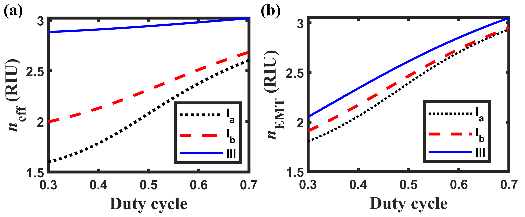
\includegraphics{Fig_sample.pdf}
		\centering
		\caption{\label{fig:MMWBGdelw}Simulated filtering responses using 3-D FDTD method 
                for $\lambda_\text{ch} = 1.27$~\mum in terms of 
                $\Lambda_\text{ch} = 392$~nm and different maximum width corrugations $\Delta w$.}
	\end{figure}
    Blah, Blah, Blah, Blah, Blah, Blah, Blah, Blah, Blah, Blah, Blah, Blah, Blah, Blah, Blah, Blah, Blah, Blah, 
    Blah, Blah, Blah, Blah, Blah, Blah, Blah, Blah, Blah, Blah, Blah, Blah, Blah, Blah, Blah, Blah, Blah, Blah, 
    Blah, Blah, Blah, Blah, Blah, Blah, Blah, Blah, Blah, Blah, Blah, Blah, Blah, Blah, Blah, Blah, Blah, Blah, 
    Blah, Blah, Blah, Blah, Blah, Blah, Blah, Blah, Blah, Blah, Blah, Blah, Blah, Blah, Blah, Blah, Blah, Blah, 
    Blah, Blah, Blah, Blah, Blah, Blah, Blah, Blah, Blah, Blah, Blah, Blah, Blah, Blah, Blah, Blah, Blah, Blah, 
    Blah, Blah, Blah, Blah, Blah, Blah, Blah, Blah, Blah, Blah, Blah, Blah, Blah, Blah, Blah, Blah, Blah, Blah, 
    Blah, Blah, Blah, Blah, Blah, Blah, Blah, Blah, Blah, Blah, Blah, Blah, Blah, Blah, Blah, Blah, Blah, Blah, 
    amplitude apodization shown in Fig.~\ref{fig:MMWBGsche}(b) are \ur{determined} to \ur{satisfy} 
    $\lambda$\SB{r} = $\lambda$\SB{ch}, 
    \begin{figure}[!t]
		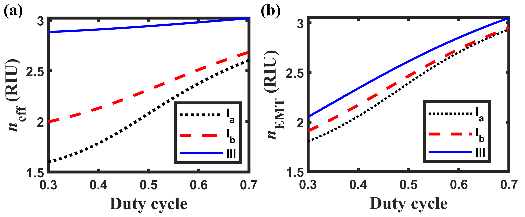
\includegraphics{Fig_sample.pdf}
		\centering
		\caption{\label{fig:MMWBGs}Simulated filtering responses 
                \rur{of \textbf{(a)} the contra-directional coupled TE\SB{1} mode, 
                \textbf{(b)} the remaining forward TE\SB{0} mode, and 
                \textbf{(c)--(f)} the} electric-field top-view profiles at the given four channel     
                wavelengths, respectively, 
                for the corresponding \rur{individual} MMWBGs using the 3-D FDTD solutions in terms of 
                the parameter set ($W$,~$\Delta w$,~\textit{s}) = (950~nm,~65~nm,~5).}
	\end{figure}
    \begin{figure}[!t]
		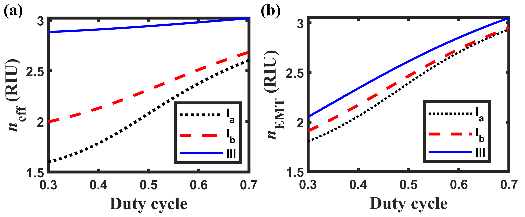
\includegraphics{Fig_sample.pdf}
		\centering
		\caption{\label{fig:BADCsche}Schematic top view of the SiN\SB{x}-based BADC for broadband coupling 
                    from the TE\SB{1} mode at through port to the TE\SB{0} mode at cross port.}
	\end{figure}
    Blah, Blah, Blah, Blah, Blah, Blah, Blah, Blah, Blah, Blah, Blah, Blah, Blah, Blah, Blah, Blah, Blah, Blah, 
    Blah, Blah, Blah, Blah, Blah, Blah, Blah, Blah, Blah, Blah, Blah, Blah, Blah, Blah, Blah, Blah, Blah, Blah, 
    Blah, Blah, Blah, Blah, Blah, Blah, Blah, Blah, Blah, Blah, Blah, Blah, Blah, Blah, Blah, Blah, Blah, Blah, 
    Blah, Blah, Blah, Blah, Blah, Blah, Blah, Blah, Blah, Blah, Blah, Blah, Blah, Blah, Blah, Blah, Blah, Blah, 
    Blah, Blah, Blah, Blah, Blah, Blah, Blah\cite{hqp-1}, Blah, Blah, Blah, Blah, Blah, Blah, Blah, Blah, Blah, Blah, Blah, 
    Blah, Blah, Blah, Blah, Blah, Blah, Blah, Blah, Blah, Blah, Blah, Blah, Blah, Blah, Blah, Blah, Blah, Blah, 
    Blah, Blah, Blah, Blah, Blah, Blah, Blah, Blah, Blah, Blah, Blah, Blah, Blah, Blah, Blah, Blah, Blah, Blah, 
    
    Blah, Blah, Blah, Blah, Blah, Blah, Blah, Blah, Blah, Blah, Blah, Blah, Blah, Blah, Blah, Blah, Blah, Blah, 
    Blah, Blah, Blah, Blah, Blah, Blah, Blah, Blah, Blah, Blah, Blah, Blah, Blah, Blah, Blah, Blah, Blah, Blah, 
    Blah, Blah, Blah, Blah, Blah, Blah, Blah, Blah, Blah, Blah, Blah, Blah, Blah, Blah, Blah, Blah, Blah, Blah, 
    Blah, Blah, Blah, Blah, Blah, Blah, Blah, Blah, Blah, Blah, Blah, Blah, Blah, Blah, Blah, Blah, Blah, Blah, 
    Blah, Blah, Blah, Blah, Blah, Blah, Blah, Blah, Blah, Blah, Blah, Blah, Blah, Blah, Blah, Blah, Blah, Blah, 
    Blah, Blah, Blah, Blah, Blah, Blah, Blah, Blah, Blah, Blah, Blah, Blah, Blah, Blah, Blah, Blah, Blah, Blah, 
    Blah, Blah, Blah, Blah, Blah, Blah, Blah, Blah, Blah, Blah, Blah, Blah, Blah, Blah, Blah, Blah, Blah, Blah, 
    
    Blah, Blah, Blah, Blah, Blah, Blah, Blah, Blah, Blah, Blah, Blah, Blah, Blah, Blah, Blah, Blah, Blah, Blah, 
    Blah, Blah, Blah, Blah, Blah, Blah, Blah, Blah, Blah, Blah, Blah, Blah, Blah, Blah, Blah, Blah, Blah, Blah, 
    Blah, Blah, Blah, Blah, Blah, Blah, Blah, Blah, Blah, Blah, Blah, Blah, Blah, Blah, Blah, Blah, Blah, Blah, 
    Blah, Blah, Blah, Blah, Blah, Blah, Blah, Blah, Blah, Blah, Blah, Blah, Blah, Blah, Blah, Blah, Blah, Blah, 
    Blah, Blah, Blah, Blah, Blah, Blah, Blah, Blah, Blah, Blah, Blah, Blah, Blah, Blah, Blah, Blah, Blah, Blah, 
    Blah, Blah, Blah, Blah, Blah, Blah, Blah, Blah, Blah, Blah, Blah, Blah, Blah, Blah, Blah, Blah, Blah, Blah, 
    Blah, Blah, Blah, Blah, Blah, Blah, Blah, Blah, Blah, Blah, Blah, Blah, Blah, Blah, Blah, Blah, Blah, Blah, 
    \begin{table}[!t]
		\caption{\label{tab:three}
		Performance comparison of CWDM filters in the literature.}
		\centering
		% \begin{ruledtabular}
		% \begin{tabular}{|P{0.6in}|P{0.45in}|P{0.45in}|P{0.45in}|P{0.45in}|P{0.45in}|}	\hline
		\begin{tabular}{|M{0.45in}|M{0.27in}|M{0.25in}|M{0.2in}|M{0.3in}|M{0.4in}|M{0.4in}|}	\hline % well fit for IEEE
			\rowcolor{lightgray}\textbf{Structure} & 
            \textbf{Blah\SB{a}} & 
            \textbf{Blah} & 
            \textbf{Blah} & 
            \textbf{Blah} & 
            \rur{\textbf{Blah}} & 
            \rur{\textbf{Blah}} \\ \hline
            
            Blah, Blah, Blah, Blah & 
                    5--6 & $-$27 & InP/ O & 3 & \rur{$<$ 3} & \rur{--} \\ \hline
            Blah, Blah, Blah, Blah & 
                    $\sim$3 & $-$25 & Si/ O & $\sim$11 & \rur{$\sim$12.8} & \rur{--} \\ \hline
            Blah, Blah, Blah, Blah & 
                    $\sim$3 & $-$2\rur{2} & Si/ C & $\sim$5.7 & \rur{$\sim$7.5} & \rur{--} \\ \hline
            Blah, Blah, Blah, Blah  & 
                    2--3 & $-$30 & SiN/ O & $\sim$6.7 & \rur{5.7} & \rur{$<$ 3} \\ \hline
            \ur{Proposed Structure} & 
                    $<$ \rur{1} & \rur{\textbf{$-$28}} & SiN/ O & \rur{\textbf{13.45}} & \rur{\textbf{$\sim$15.7}} & \rur{\textbf{14.35}} \\ \hline
		\end{tabular}
		% \end{ruledtabular}
        \begin{flushleft}
			\SP{a} 1-dB bandwidth measured from \ur{the} transmission peak.\\	
			% \rur{\SP{b} Available bandwidth for channel XT below $-$20~dB, \textit{i.e.}, ABW\SB{20-dB}.}\\	
			% \rur{\SP{c}} Available bandwidth for channel XT below $-$2\rur{8}~dB, \textit{i.e.}, ABW\SB{2\rur{8}-dB}.\\	
			% \SP{d} Echelle grating; \SP{e} Multi-mode interferometer; \SP{f} Waveguide Bragg grating. \\
		\end{flushleft}
	\end{table}
    Blah, Blah, Blah, Blah, Blah, Blah, Blah, Blah, Blah, Blah, Blah, Blah, Blah, Blah, Blah, Blah, Blah, Blah, 
    Blah, Blah, Blah, Blah, Blah, Blah, Blah, Blah, Blah, Blah, Blah, Blah, Blah, Blah, Blah, Blah, Blah, Blah, 
    Blah, Blah, Blah, Blah, Blah, Blah, Blah, Blah, Blah, Blah, Blah, Blah, Blah, Blah, Blah, Blah, Blah, Blah, 
    Blah, Blah, Blah, Blah, Blah, Blah, Blah, Blah, Blah, Blah, Blah, Blah, Blah, Blah, Blah, Blah, Blah, Blah, 
    Blah, Blah, Blah, Blah, Blah, Blah, Blah, Blah, Blah, Blah, Blah, Blah, Blah, Blah, Blah, Blah, Blah, Blah, 
    Blah, Blah, Blah, Blah, Blah, Blah, Blah, Blah, Blah, Blah, Blah, Blah, Blah, Blah, Blah, Blah, Blah, Blah, 
    Blah, Blah, Blah, Blah, Blah, Blah, Blah, Blah, Blah, Blah, Blah, Blah, Blah, Blah, Blah, Blah, Blah, Blah, 

\section{Analysis of fabrication tolerance}
\label{sec:three}
    \begin{figure}[!t]
		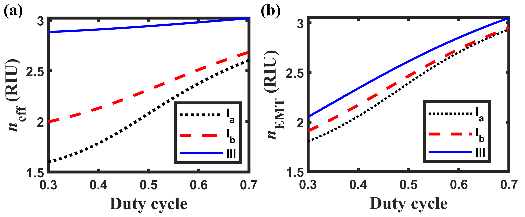
\includegraphics{Fig_sample.pdf}
		\centering
		\caption{\label{fig:MMWBGtole}Simulated filtering responses \rur{of the individual MMWBGs} 
                    using 3-D FDTD method at \rur{the} four channels 
                    in terms of \rur{the configuration in Fig.~\ref{fig:MMWBGsche}} and 
                    the \rur{given} over-etching errors $W_\text{e}$ \rur{within ($\pm$18~nm)} with a step of 6~nm.}
	\end{figure}
    Blah, Blah, Blah, Blah, Blah, Blah, Blah, Blah, Blah, Blah, Blah, Blah, Blah, Blah, Blah, Blah, Blah, Blah, 
    Blah, Blah, Blah, Blah, Blah, Blah, Blah, Blah, Blah, Blah, Blah, Blah, Blah, Blah, Blah, Blah, Blah, Blah, 
    Blah, Blah, Blah, Blah, Blah, Blah, Blah, Blah, Blah, Blah, Blah, Blah, Blah, Blah, Blah, Blah, Blah, Blah, 
    Blah, Blah, Blah, Blah, Blah, Blah, Blah, Blah, Blah, Blah, Blah, Blah, Blah, Blah, Blah, Blah, Blah, Blah, 
    Blah, Blah, Blah, Blah, Blah, Blah, Blah, Blah, Blah, Blah, Blah, Blah, Blah, Blah, Blah, Blah, Blah, Blah, 
    Blah, Blah, Blah, Blah, Blah, Blah, Blah, Blah, Blah, Blah, Blah, Blah, Blah, Blah, Blah, Blah, Blah, Blah, 
    Blah, Blah, Blah, Blah, Blah, Blah, Blah, Blah, Blah, Blah, Blah, Blah, Blah, Blah, Blah, Blah, Blah, Blah, 
 
\section{Conclusion\ur{s}}
\label{sec:four}
    Blah, Blah, Blah, Blah, Blah, Blah, Blah, Blah, Blah, Blah, Blah, Blah, Blah, Blah, Blah, Blah, Blah, Blah, 
    Blah, Blah, Blah, Blah, Blah, Blah, Blah, Blah, Blah, Blah, Blah, Blah, Blah, Blah, Blah, Blah, Blah, Blah, 
    Blah, Blah, Blah, Blah, Blah, Blah, Blah, Blah, Blah, Blah, Blah, Blah, Blah, Blah, Blah, Blah, Blah, Blah, 
    Blah, Blah, Blah, Blah, Blah, Blah, Blah, Blah, Blah, Blah, Blah, Blah, Blah, Blah, Blah, Blah, Blah, Blah, 
    Blah, Blah, Blah, Blah, Blah, Blah, Blah, Blah, Blah, Blah, Blah, Blah, Blah, Blah, Blah, Blah, Blah, Blah, 
    Blah, Blah, Blah, Blah, Blah, Blah, Blah, Blah, Blah, Blah, Blah, Blah, Blah, Blah, Blah, Blah, Blah, Blah, 
    Blah, Blah, Blah, Blah, Blah, Blah, Blah, Blah, Blah, Blah, Blah, Blah, Blah, Blah, Blah, Blah, Blah, Blah, 

\rur{
\section*{Acknowledgments}
	The authors are thankful to Blah, Blah, Blah, Blah, Blah, Blah, Blah, Blah, Blah, Blah, Blah, Blah, Blah, Blah, Blah, Blah, Blah, Blah, 
    Blah, Blah, Blah, Blah, Blah, Blah, Blah, Blah, Blah, Blah, Blah, Blah, Blah, Blah, Blah, Blah, Blah, Blah.}

\bibliographystyle{IEEEtranDOI}
\bibliography{IEEEuabrv,main_IEEE_PJ}

\end{document}


